% ==========================================
% BAB II STUDI LITERATUR
% ==========================================
\chapter{STUDI LITERATUR}
\label{chap:studi-literatur}
Bab studi literatur menjelaskan kajian-kajian yang relevan dengan permasalahan yang diangkat
pada tugas akhir ini. Penjelasan dalam bab ini akan mencakup tinjauan terhadap karhutla dan
penerapan model \textit{Machine Learning} (ML) serta XAI, dan literatur terkait seputar 
solusi prediktif terhadap bencana karhutla. Kajian yang dilakukan berguna untuk memberikan 
pemahaman dan landasan dalam memahami domain dan menerapkan solusi yang relevan.
\section{Kebakaran Hutan dan Lahan (Karhutla) di Indonesia}
Kebakaran hutan dan lahan (karhutla) merupakan kejadian berkobarnya api yang meliputi
hutan serta lahan gambut/mineral yang sering dipicu oleh kombinasi faktor antropogenik
dan kondisi lingkungan serta dapat terjadi dengan frekuensi tahunan \autocite{Nurhayati2021}.
Peristiwa ini menjadi ancaman berulang di Indonesia, salah satunya di wilayah Kalimantan.
Dampak yang ditimbulkan oleh karhutla mengakibatkan kerusakan hingga ke berbagai aspek: 
\begin{enumerate}
    \item Kerusakan Ekologis: Karhutla menyebabkan kerusakan lahan serta menjadi bencana yang menimbulkan hilangnya biodiversitas dan menyebabkan pemanasan global \autocite{Thoha2021}.
    \item Dampak Kesehatan: Asap lintas batas (\textit{transboundary haze}) yang dihasilkan membawa partikel aerosol berbahaya (PM\textsubscript{2.5}) yang terbukti secara klinis menyebabkan peningkatan signifikan pada kasus infeksi saluran pernapasan akut (ISPA), asma, dan bahkan kematian prematur pada populasi yang terpapar \autocite{syahid2022}.
    \item Kerugian Ekonomi: Bank Dunia memperkirakan kerugian ekonomi akibat karhutla pada tahun 2019 saja mencapai 5,2 miliar USD di Indonesia, setara dengan 0,5\% dari PDB negara. Kerugian ini mencakup kerusakan pada sektor pertanian, kehutanan, transportasi, dan pariwisata, serta biaya pemadaman yang sangat besar \autocite{jain2021}.
\end{enumerate}
\section{Faktor Pemicu Karhutla}
Penyebab karhutla di Indonesia umumnya disebabkan hasil interaksi antara kondisi lingkungan yang membuat hutan dan lahan menjadi rentan 
dan aktivitas manusia yang menyulut api. Sejumlah studi mengatakan bahwa variabilitas dari iklim (seperti ENSO dan kekeringan), karakteristik
biofisik (keberadaan lahan gambut), serta faktor antropogenik (aktivitas manusia) saling memperkuat satu sama lain dalam membentuk pola
karhutla di Indonesia. 
\subsection{Faktor Meteorologis}
Faktor meteorologis berperan sebagai pemicu yang menentukan seberapa mudah suatu daerah terbakar. Cuaca dan musim merupakan faktor yang dapat mempengaruhi 
kondisi lingkungan. Sejumlah penelitian juga menunjukkan bahwa anomali iklim berkaitan kuat dengan intensitas kebakaran di Indonesia. Studi oleh \textcite{Fitriany2021}
menemukan bahwa kejadian kebakaran hutan di Indonesia berkorelasi dengan indeks iklim jangka panjang seperti El Niño-Southern Oscillation (ENSO) dan Indian Ocean Dipole (IOD). 
ENSO sendiri memiliki dua fase yang mempengaruhi kondisi iklim lingkungan. 
\begin{enumerate}
  \item El Niño: Fenomena ini secara signifikan mengurangi curah hujan dan memperpanjang durasi musim kemarau di sebagian besar wilayah Indonesia \autocite{syahid2022}. Analisis 
  data historis menunjukkan korelasi positif yang kuat antara indeks ENSO dan jumlah \textit{hotspot} (titik deteksi kebakaran) 
  yang terdeteksi oleh satelit. Selama episode El Niño yang kuat, penurunan kelembapan tanah 
  dan vegetasi menciptakan kondisi lingkungan yang sangat kondusif bagi penyebaran api yang cepat dan luas.
  \item La Niña: Sebaliknya, La Niña membawa kondisi yang lebih basah  ke Indonesia, yang secara efektif 
  menekan aktivitas kebakaran dan mengurangi jumlah \textit{hotspot} tahunan \autocite{syahid2022}. Siklus ENSO 
  ini menjelaskan mengapa intensitas Karhutla di Indonesia sangat berfluktuasi dari tahun ke tahun.
\end{enumerate}

\subsection{Faktor Antropogenik}
Walaupun iklim menciptakan kondisi yang rentan, sebagian besar api awal (\textit{ignition}) di Indonesia justru berasal dari aktivitas manusia, 
bukan penyebab alami. Faktor antropogenik merupakan faktor yang berhubungan dengan aktivitas manusia.
Sejumlah kajian menunjukkan bahwa pemicu utama karhutla di Indonesia didominasi oleh aktivitas manusia. \textcite{Nurhayati2021} menemukan bahwa pola
kebakaran di lahan gambut Sumatra banyak terjadi di kawasan dengan tekanan pemanfaatan lahan tinggi. Sementara itu, menurut 
\textcite{Rossita2023} kebakaran berulang yang terjadi di Riau berhubungan dengan praktik pengelolaan lahan dan drainase. Temuan-temuan ini
menegaskan bahwa faktor sosial dan tata kelola lahan berkontribusi besar terhadap peningkatan frekuensi bencana karhutla.

\subsection{Faktor Biofisik}
Faktor biofisik berkaitan dengan karakteristik fisik dan wilayah ekologis yang memengaruhi kerentanan suatu area terhadap kebakaran. 
Beberapa faktor utama yang banyak dibahas dalam literatur antara lain keberadaan lahan gambut, jenis tutupan lahan (vegetasi), dan topografi. 
\textcite{Rossita2023} menunjukkan bahwa gambut mencakup sekitar 8\% dari luas daratan Indonesia, dan analisis mereka di satu kesatuan hidrologis gambut 
di Riau menemukan tren peningkatan luas gambut terbakar antara 2001-2020, dengan sekitar 33\% area yang terbakar mengalami kebakaran berulang. 
Hal ini mengindikasikan perangkap degradasi, di mana lahan yang pernah terbakar menjadi semakin rentan untuk terbakar kembali pada tahun-tahun berikutnya.

\section{Indeks Cuaca Kebakaran}
Salah satu pendekatan yang banyak digunakan untuk menilai tingkat bahaya kebakaran karhutla adalah Fire Weather Index (FWI). Studi oleh \textcite{NurFitriani2023} 
menjelaskan bahwa FWI menjadi dasar dari Fire Danger Rating System (FDRS) yang dioperasikan oleh BMKG untuk memantau potensi bahaya karhutla secara harian. Sistem ini 
menggabungkan informasi cuaca harian bahaya karhutla seperti suhu, kelembapan, kecepatan angin, dan curah hujan untuk menghasilkan indeks
yang menggambarkan tingkat risiko kebakaran di suatu wilayah.

\textcite{NurFitriani2023} bahwa FDRS Indonesia telah disesuaikan dengan sistem FWI yang awalnya dikembangkan di Kanada dan kemudian diadaptasi untuk 
kondisi iklim di Indonesia. Dalam sistem ini, indeks FWI terdiri dari enam komponen yang dibagi menjadi dua kelompok utama, yaitu kode kelembapan bahan bakar (\textit{fuel moisture codes})
dan indeks perilaku kebakaran (\textit{fire behaviour indices}).
\begin{enumerate}
  \item Fine Fuel Moisture Code (FFMC) \\
  Menggambarkan kelembapan lapisan permukaan atas tanah dan bahan bakar yang sangat halus seperti ranting kecil. Nilai FFMC yang tinggi menunjukkan kondisi bahan bakar permukaan sangat kering 
  sehingga mudah terbakar.
  \item Duff Moisture Code (DMC) \\
  Menggambarkan kelembapan lapisan bahan organik pada kedalaman menengah di bawah permukaan tanah. Kode ini peka terhadap kekeringan pada skala mingguan
  \item Drought Code (DC) \\
  Menggambarkan kelembapan lapisan bahan organik yang lebih dalam dan berhubungan dengan kekeringan jangka panjang. Nilai DC yang tinggi menandakan kondisi sangat kering dan potensi kebakaran
  bawah permukaan yang sulit dipadamkan
  \item Initial Spread Index (ISI) \\
  Merupakan indeks yang menggabungkan FFMC dan kecepatan angin untuk memperkirakan laju awal penjalaran api jika terjadi penyalaan. Semakin kering bahan bakar dan semakin kencang angin, semakin besar nilai ISI.
  \item Build-Up Index (BUI) \\
  Menggabungkan DMC dan DC untuk merepresentasikan akumulasi bahan bakar kering yang tersedia. BUI yang besar menunjukkan banyaknya bahan bakar yang siap dikonsumsi api.
  \item Fire Weather Index (FWI) \\
  Merupakan indeks utama yang diperoleh dari kombinasi ISI dan BUI dan digunakan sebagai indikator intensitas potensial kebakaran hutan dan lahan. Menurut penjelasan pada laman resmi BMKG, FWI menunjukkan besarnya
  intensitas api jika terjadi kebakaran dan sangat dipengaruhi nilai ISI dan BUI.
\end{enumerate}
Laman resmi BMKG menyajikan peta FWI dan indeks terkait dalam bentuk peta spasial untuk melihat beberapa kategori tingkat bahaya untuk membantu kepentingan dalam memantau
potensi kebakaran pada skala nasional. FWI dipandang sebagai kerangka indeks bahaya berbasis cuaca yang sudah teruji dan digunakan secara operasional di Indonesia. Namun, pendekatan ini
berfokus ke variabel meteorologis, sedangkan banyak penelitian yang menunjukkan bahwa risiko karhutla ternyata dipengaruhi oleh banyak faktor selain meteorologis.


\section{\textit{Artificial Intelligence}}
\textit{Artificial Intelligence} (AI) adalah bidang ilmu komputer yang luas dan berkaitan dengan pembangunan mesin pintar yang mampu melakukan tugas-tugas
yang biasanya membutuhkan kecerdasan manusia \autocite{Sarker2022}. Penelitian ini juga menjelaskan bahwa AI berhasil mentransformasikan 
sebagian besar industri, mulai dari keuangan dan manufaktur hingga transportasi. AI membantu manusia dalam mengambil keputusan dengan berperan sebagai 
sistem yang dapat mengolah data dalam jumlah besar, mengekstraksi pola, dan menghasilkan prediksi atau rekomendasi untuk mendukung pengambilan keputusan. 
\textcite{Gupta2022} menjelaskan bahwa integrasi AI dan \textit{big data} telah menjadi fondasi utama sistem pengambilan keputusan berbasis data di berbagai sektor untuk saat ini.
 Pada tugas akhir, peran AI relevan dalam tindakan prediksi risiko kebakaran hutan serta penyajian informasi untuk membantu
pengelola karhutla dalam menetapkan langkah mitigasi.

\begin{figure}[h] % pilihan opsi yang disarankan: t = top, b = bottom, h = here
	\centering
  \captionsetup{justification=centering}
    	\includegraphics[width=1\textwidth]{image/hierarki-AI.png}
	\caption{Ilustrasi posisi hierarki ML dan DL pada area AI \autocite{Sarker2022}}
	\label{gambar:hierarki-AI}
\end{figure}


\textit{Artificial Intelligence}, \textit{Machine Learning} (ML), dan \textit{Deep Learning} (DL)
saling berkaitan secara hierarkis seperti yang ditunjukkan pada Gambar \ref{gambar:hierarki-AI} dan berinteraksi dalam membangun sistem perangkat lunak
yang cerdas. Menurut \textcite{Sarker2022}, ML dan DL merupakan bagian dari teknologi AI yang
berfokus pada pembelajaran berbasis data untuk mengembangkan sistem cerdas dan
mengotomatisasi proses. DL sendiri merupakan subbagian ML yang memanfaatkan jaringan
saraf berlapis untuk mempelajari representasi yang kompleks, sehingga berperan penting dalam
analitik tingkat lanjut dan pengambilan keputusan cerdas.

\section{\textit{Machine Learning}}
\textit{Machine Learning} (ML) merupakan cabang utama dari AI yang berfokus pada bagaimana komputer dapat
belajar dari data untuk meningkatkan kinerja tugas tertentu tanpa diprogram secara eksplisit untuk setiap
aturan. Menurut \textcite{Sarker2021}, ML telah berkembang pesat dalam konteks analisis
data dan komputasi serta meningkatkan pengalaman otomatisasi dan mendorong revolusi industri keempat (Industri 4.0).
Dalam AI, ML telah muncul sebagai metode pilihan untuk mengembangkan perangkat lunak praktis untuk
visi komputer, pengenalan suara, pemrosesan bahasa alami, kendali robot, dan lainnya.

\begin{figure}[h] % pilihan opsi yang disarankan: t = top, b = bottom, h = here
	\centering
  \captionsetup{justification=centering}
    	\includegraphics[width=1\textwidth]{image/struktur-machine-learning.png}
	\caption{Struktur umum ML pada fase pelatihan dan pengujian \autocite{Sarker2022}}
	\label{gambar:struktur ML}
\end{figure}

Dalam konteks organisasi, \textcite{Gupta2022} menunjukkan bahwa pemanfaatan model ML yang didasari oleh infrastruktur \textit{big data} mampu meningkatkan
kualitas pengambilan keputusan melalui hasil prediksi, klasifikasi, atau deteksi pola anomali yang lebih akurat dibandingkan 
pendekatan konvensional. Pada Gambar \ref{gambar:struktur ML}, kerangka umum model prediktif berbasis ML ditandai dengan dua fase sebelum menjadi sebuah model prediktif. 
Kerangka model ML diawali dengan fase 1, yaitu pelatihan dari data historis dan menghasilkan prediksi untuk dijadikan sebagai data uji pada
fase 2. Secara garis besar, \textcite{Sarker2022} membagi ML ke dalam tiga kategori utama, yaitu \textit{supervised learning}, 
\textit{unsupervised learning}, dan \textit{reinforcement learning}.

Pada \textit{supervised learning}, model dilatih dengan fitur masukan dan label sehingga dapat melakukan prediksi pada data baru yang
belum pernah dilihat. Pendekatan ini sangat relevan dengan prediksi risiko karhutla karena data historis sudah mencatat faktor-faktor 
yang menyebabkan suatu lokasi kebakaran atau tidak. \textit{Unsupervised learning} digunakan ketika label tidak tersedia dan model berfokus
dalam menemukan pola atau struktur tersembunyi. Disebabkan data tidak memiliki label, model harus bisa memprediksi pola menggunakan metode
seperti \textit{clustering}. Terdapat model yang menggabungkan antara \textit{supervised} dan \textit{unsupervised} bernama \textit{semi-supervised learning} yang biasa digunakan ketika jumlah data berlabel tidak cukup banyak sehingga memanfaatkan data tidak berlabel untuk memperkaya data.
\textit{Reinforcement learning} mempelajari strategi atau tindakan terbaik melalui interaksi dengan lingkungan dan umpan balik berupa \textit{reward} atau \textit{penalty}.
Model ini lebih relevan untuk digunakan pada sistem kontrol atau penjadwalan dinamis pada pemodelan risiko statis.

\begin{table}[t] % pilihan opsi yang disarankan: t = top, b = bottom, h = here
  \begin{tabular}{| p{3cm} | p{5cm} | p{4cm} |}
    \hline
    Tipe pembelajaran & Proses pembentukan model & Tugas umum \\
    \hline
    \textit{Supervised learning} &
    Algoritma atau model belajar dari data berlabel (pendekatan berbasis tugas) &
    Klasifikasi, Regresi \\
    \hline
    \textit{Unsupervised learning} &
    Algoritma atau model belajar dari data tidak berlabel (pendekatan berbasis data) &
    Klastering, Asosiasi, Reduksi dimensi \\
    \hline
    \textit{Semi-supervised learning} &
    Model dibangun menggunakan kombinasi data berlabel dan tidak berlabel &
    Klasifikasi, Klastering \\
    \hline
    \textit{Reinforcement learning} &
    Model belajar berdasarkan \textit{reward} atau penalti (pendekatan berbasis lingkungan) &
    Klasifikasi, Kontrol \\
    \hline
  \end{tabular}
  \caption{Kategori \textit{Machine Learning} \autocite{Sarker2022}}
  \label{tbl:tipe-pembelajaran-ml}
\end{table}

\subsection{Konsep \textit{Supervised Learning}}
\textcite{Sarker2021} mendefinisikan \textit{supervised learning} sebagai pendekatan ML sebagai model yang belajar dari data
yang sudah memiliki label. Setiap contoh data terdiri atas pasangan masukan dan keluaran yang benar sehingga model dapat 
mempelajari pemetaan dari fitur-fitur pada data hingga ke label berdasarkan seluruh contoh data tersebut. Pendekatan ini 
banyak digunakan pada tugas klasifikasi dan regresi di berbagai domain karena secara langsung memanfaatkan informasi target
yang diketahui saat pelatihan. 

Secara matematis, data latih pada \textit{supervised learning} dapat dituliskan sebagai 
\begin{equation}
D = \{(x_1, y_1), (x_2, y_2), ..., (x_n,y_n)\}
\label{eq:himpunan-data-supervised-learning}
\end{equation}

Pada Persamaan \ref{eq:himpunan-data-supervised-learning}, $x_i \in \mathbb{R}^d$ merupakan vektor fitur untuk contoh ke ke-$i$, dan $y_i$ yang merupakan label atau nilai
target yang bersesuaian. Pada \textit{supervised learning}, kesalahan yang dimiliki model akan menjadi hukuman dan semakin besar kesalahannya akan semakin
besar hukumannya. Jadi, tugas utama \textit{supervised learning} adalah memilih suatu model ($f(x;\theta)$) dan kemudian mencari parameter
$theta$ yang membuat hasil model dapat sedekat mungkin dengan label yang benar.
Untuk menilai seberapa bagus model tersebut, terdapat fungsi kerugian yang dapat mengukur seberapa jauh prediksi dari label sebenarnya.
\begin{equation}
R^{(\theta)} = \frac{1}{n} \sum_{i=1}^{n} L\!\left( y_i,\, f(x_i;\theta) \right)
\label{eq:empirical-risk}
\end{equation}
Rata-rata kerugian pada seluruh data latih (\textit{empirical risk}) dinyatakan pada Persamaan \ref{eq:empirical-risk}. Secara konsep, proses pelatihan model \textit{supervised learning} dapat dipahami sebagai upaya pencarian nilai $theta$ yang dapat meminimalkan
kerugian rata-rata.
\subsection{\textit{Linear Regression}}
\textit{Linear regression} (LR) adalah contoh paling sederhana dan klasik dari model \textit{supervised learning}. Model ini
menggambarkan hubungan antara sekumpulan fitur dan suatu nilai keluaran secara kontinu dengan menggambar garis lurus
(untuk satu fitur) atau bidang (untuk banyak fitur). Pada Persamaan \ref{eq:linear-regression-formula}, $\beta_0$ merupakan titik potong dengan sumbu vertikal dan setiap $beta_j$ menunjukkan 
seberapa besar kontribusi suatu fitur $x_j$ terhadap perubahan nilai \textit{output} $y$. Istilah 
$\varepsilon$ digunakan sebagai galat karena terdapat variasi yang bisa saja tidak bisa dijelaskan oleh kombinasi
linier dari fitur-fitur tersebut.
\begin{equation}
y = \beta_0 + \beta_1 x_1 + \beta_2 x_2 + \cdots + \beta_k x_k + \varepsilon.
\label{eq:linear-regression-formula}
\end{equation}
\subsection{\textit{Random Forest}}
\begin{figure}[h] % pilihan opsi yang disarankan: t = top, b = bottom, h = here
	\centering
  \captionsetup{justification=centering}
    	\includegraphics[width=1\textwidth]{image/struktur-random-forest.png}
	\caption{Stuktur model \textit(Random Forest) \autocite{Sarker2021}}
	\label{gambar:sturktur-rf}
\end{figure}
\textit{Random Forest} (RF) adalah pendekatan ML yang menggabungkan prediksi beberapa pohon keputusan untuk menciptakan model
yang lebih tangguh dan akurat. Dengan melakukan akumulasi keluaran melalui teknik seperti pemungutan suara (untuk klasifikasi)
atau \textit{averaging} (untuk regresi), RF dapat meningkatkan kemampuan prediksinya dan meminimalkan terjadinya \textit{overfitting} \autocite{Karurung2025}.
Selain itu, menurut \textcite{Sarker2021} setiap pohon pada RF dilatih dengan sampel data yang berbeda dan hanya melihat subset acak 
dari fitur pada setiap pemisahan. Hal ini mengakibatkan masing-masing pohon dapat belajar pola yang berbeda sehingga kesalahan yang
dibuat satu pohon dapat dikoreksi ketika digabungkan dengan pohon lain.
\begin{equation}
\hat{y} = \mathrm{mode}\big(h_1(x),\, h_2(x),\, \ldots,\, h_K(x)\big)\
\label{eq:rf-formula}
\end{equation}

Pada langkah prediksi untuk tugas klasifikasi, RF melakukan langkah \textit{majority vote} dalam memilih keluaran. Pada Persamaan \ref{eq:rf-formula}, metode \textit{majority vote} 
ditentukan dengan memilih kelas mana yang paling sering dipilih dari seluruh pohon. Pendekatan ini membantu mengurangi varians yang biasanya muncul pada satu pohon keputusan saja
sekaligus meningkatkan akurasi model. Selain menghasilkan prediksi kelas risiko, RF juga menyediakan ukuran pentingnya suatu fitur \textit{feature importance} yang dapat
dimanfaatkan sebagai awal bagi analisis \textit{explainable AI} yang lebih mendalam.
\subsection{\textit{Extreme Gradient Boosting}}
XGBoost (\textit{Extreme Gradient Boosting}) merupakan algoritma \textit{gradient boosting} berbasis pohon keputusan yang banyak digunakan
dalam studi prediksi karena menggabungkan kinerja prediksi yang tinggi dengan efisiensi komputasi serta mampu menangani data dalam skala besar.
Berbeda dengan RF, XGBoost menyusun pohon secara bertahap untuk memperbaiki kesalahan model sebelumnya. \textcite{Wiens2025} menyebutkan persamaan
prediksi XGBoost untuk contoh ke-$i$ sebagai penjumlahan keluaran dari $big(K)$ pohon sebagai berikut.
\begin{equation}
F_k(x) = F_0(x) + \varepsilon T_1(x) + \varepsilon T_2(x) + \dots + \varepsilon T_k(x)\
\label{eq:xgboost-formula}
\end{equation}
Pada Persamaan~\ref{eq:xgboost-formula}, $F_0(x)$ biasanya berupa model awal 
sederhana (misalnya nilai rata-rata), $T_m(x)$ merepresentasikan pohon regresi 
pada iterasi ke-$m$, dan $\varepsilon$ adalah \textit{learning rate} yang 
mengendalikan besar langkah pembaruan model. Hal ini sesuai dengan pendapat \textcite{Sarker2021} bahwa gradien yang digunakan pada XGBoost berguna
untuk meminimalkan fungsi kerugian yang serupa dengan cara kerja jaringan saraf tiruan (\textit{Artificial Neural Network}).
\section{Metrik Evaluasi}
Dalam pengembangan model \textit{Machine Learning} untuk melakukan prediksi, langkah evaluasi sangat diperlukan untuk menilai apakah model
memiliki kemampuan yang cukup untuk memprediksi label. Langkah untuk melakukan evaluasi tersebut dapat menggunakan metrik evaluasi 
untuk melihat kinerja dan performa model. Jenis metrik evaluasi yang dapat digunakan sebagai bahan evaluatif berbeda-beda setiap modelnya dengan
mempertimbangkan sifat data, jenis tugas, dan kebutuhan interpretasi. Berdasarkan penjelasan dari \textcite{Miller2024}, metrik evaluasi dikelompokkan
berdasarkan informasi yang berasal dari \textit{confusion matrix}, seperti \textit{accuracy}, \textit{precision}, \textit{recall}, 
\textit{F1-score} serta metrik berbasis kurva seperti \textit{Receiver Operating Characteristic} (ROC) dan \textit{Area Under the Curve} (AUC).

Pada konteks karhutla sendiri, berbagai studi menunjukkan penggunaan metrik yang berbeda-beda tergantung cara mereka melakukan prediksi dan jenis
model prediksi yang digunakan. Walaupun begitu, setiap studi menggunakan kombinasi metrik untuk memberikan evaluasi model secara jelas. Penelitian 
yang dilakukan \textcite{Abdollahi2023} menggunakan metrik akurasi, \textit{precision}, \textit{recall}, \textit{F1-Score}, dan AUC-ROC dalam melakukan
evaluasi model \textit{wildfire susceptibility} dan menilai kemampuan model dari berbagai sudut pandang. Di sisi lain, studi dari \textcite{Karurung2025}
memanfaatkan metrik yang sama seperti studi sebelumnya untuk melakukan perbandingan antara model RF dan XGBoost. 
Sementara itu, studi dari \textcite{Eaturu2025} yang membandingkan model ML dan DL dalam melakukan prediksi memanfaatkan \textit{Root Mean Square Error} (RMSE), 
\textit{Mean Absolute Error} (MAE), dan $R^2$ (\textit{coefficient of determination}) untuk mengevaluasi model prediksi kebakaran di Asia Tenggara.
\subsection{\textit{Confusion Matrix}}
\textcite{Miller2024} dan \textcite{Sokolova2009} menjelaskan bahwa \textit{confusion matrix} merupakan representasi dasar untuk menilai performa model yang melakukan klasifikasi
berdasarkan rangkuman prediksi benar dan salah pada tiap kelas. Mereka juga menambahkan bahwa metode ini berfungsi untuk menjadi basis dalam perhitungan
berbagai metrik seperti \textit{accuracy}, \textit{precision}, dan \textit{recall}. Untuk contoh klasifikasi biner seperti ini, \textit{confusion matrix}
memuat empat kategori, yaitu \textit{true positive} (TP), \textit{true negative} (TN), \textit{false positive} (FP), dan \textit{false negative} (FN).
Empat kategori tersebut, dapat memberikan wawasan dan diturunkan menjadi beberapa perhitungan evaluatif.
\begin{figure}[h] % pilihan opsi yang disarankan: t = top, b = bottom, h = here
	\centering
  \captionsetup{justification=centering}
    	\includegraphics[width=1\textwidth]{image/confusion-matrix-karhutla.png}
	\caption{Contoh penerapan \textit{confusion matrix} pada kasus label data karhutla}
	\label{gambar:confusion-matrix-karhutla}
\end{figure}

\begin{enumerate}
  \item Akurasi: efektivitas keseluruhan sebuah model \textit{classifier}
  \begin{equation}
  \text{Accuracy} = \frac{TP + TN}{TP + TN + FP + FN}
  \label{eq:accuracy-formula}
  \end{equation}

  \item Precision: proporsi prediksi positif yang benar-benar positif
  \begin{equation}
  \text{Precision} = \frac{TP}{TP + FP}
  \label{eq:precision-formula}
  \end{equation}

  \item Recall (Sensitivity): kemampuan model menemukan seluruh kelas positif
  \begin{equation}
  \text{Recall} = \frac{TP}{TP + FN}
  \label{eq:recall-formula}
  \end{equation}

  \item F1-Score: rata-rata harmonik dari precision dan recall
  \begin{equation}
  \text{F1\text{-}Score} = 2 \times \frac{\text{Precision} \times \text{Recall}}{\text{Precision} + \text{Recall}}
  \label{eq:f1-formula}
  \end{equation}

  \item Specificity: kemampuan model mengidentifikasi kelas negatif dengan benar
  \begin{equation}
  \text{Specificity} = \frac{TN}{TN + FP}
  \label{eq:specificity-formula}
  \end{equation}
\end{enumerate}

Akurasi saja sering kali tidak cukup untuk menilai sebuah model, terutama ketika jumlah kelas tidak seimbang.
Dalam situasi tersebut, kombinasi metrik seperti \textit{F1-Score} atau \textit{precision-recall} lebih informatif untuk melihat kemampuan model dalam
menangkap kelas minoritas.

\subsection{Kurva ROC dan Area AUC}
\begin{figure}[h] % pilihan opsi yang disarankan: t = top, b = bottom, h = here
	\centering
  \captionsetup{justification=centering}
    	\includegraphics[width=1\textwidth]{image/roc-auc-curve.png}
	\caption{Kurva ROC dan area ROC}
	\label{gambar:auc-roc-curve}
\end{figure}
Untuk model yang menghasilkan skor probabilitas atau skor risiko, penggunaan kurva \textit{Receiver Operating Characteristic} ROC
dan \textit{Area Under the Curve} (AUC) sebagai metrik evaluasi yang tidak bergantung pada satu nilai batas saja. ROC merupakan evaluasi
yang bergantung dari nilai \textit{True Positive Rate} (TPR) terhadap \textit{False Positive Rate} (FPR) pada nilai ambang keputusan dengan persamaan
sebagai berikut.
\begin{equation}
    \text{TPR} = \frac{TP}{TP + FN},
    \label{eq:TPR-formula}
\end{equation}

\begin{equation}
    \text{FPR} = \frac{FP}{FP + TN}.
    \label{eq:FPR-formula}
\end{equation}

AUC dijelaskan sebagai luas area bawah kurva ROC yang apabila nilainya mendekati 1 model menunjukkan kemampuan pemisahan kelas dengan sangat baik.
Namun, menurut \textcite{Lavazza2025}, sebenarnya baik ROC maupun AUC secara konseptual dikembangkan untuk klasifikasi biner karena keduanya bergantung langsung pada
definisi dua kelas (positif dan negatif) melalui TPR dan FPR. Meskipun dapat diperluas menjadi multikelas, interpretasinya kurang
representif dibandingkan situasi biner. Selain itu AUC sering kali terlalu optimis pada dataset yang tidak seimbang sehingga diperlukan
untuk melakukan kombinasi metrik dalam melihat performa model. Hal ini selaras dengan penelitian yang dilakukan oleh \textcite{Karurung2025} maupun 
\textcite{Abdollahi2023} karena keduanya mengombinasikan AUC dengan metrik evaluasi lainnya.

\subsection{Metrik Regresi}
Saat label berupa nilai kontinu, metrik yang digunakan adalah metrik regresi. Dalam studi \textcite{Eaturu2025}, 
langkah evaluasi yang dilakukan adalah dengan menggunakan kombinasi RMSE, MAE, dan koefisien determinasi untuk menilai kualitas
prediksi terhadap data observasi. Secara umum, RMSE didefinisikan sebagai
\begin{equation}
\text{RMSE} = \sqrt{\frac{1}{n} \sum_{i=1}^{n} \left( \hat{y}_i - y_i \right)^2},
\label{eq:rmse-formula}
\end{equation}
dengan $y_i$ nilai aktual, $\hat{y}_i$ nilai prediksi, dan $n$ jumlah pengamatan. RMSE memberikan penalti lebih besar pada kesalahan yang besar karena
selisih dipangkatkan terlebih dahulu sebelum dirata-ratakan, sehingga sensitif terhadap \textit{outlier}. Nilai RMSE yang lebih kecil menunjukkan bahwa rata-rata selisih 
kuadrat antara prediksi dan observasi lebih rendah. Salah satu metrik lainnya yang digunakan untuk mengevaluasi label kontinu adalah MAE.
\begin{equation}
\text{MAE} = \frac{1}{n} \sum_{i=1}^{n} \left| \hat{y}_i - y_i \right|.
\label{eq:mae-formula}
\end{equation}
MAE mengukur kesalahan rata-rata dalam satuan yang sama dengan target. Berbeda dengan RMSE, MAE memberikan bobot yang sama pada setipa kesalahan sehingga
interpretasinya lebih langsung. Intinya, semakin kecil nilai MAE berarti prediksi model lebih bagus atau lebih dekat dengan nilai aktual.
\section{\textit{Explainable Artificial Intelligence} (XAI)}
Model ML seperti RF dan XGBoost sering kali mencapai akurasi tinggi dalam melakukan prediksi. Namun, seluruh model prediksi sering dianggap sebagai "\textit{black box}"
atau kotak hitam karena tidak adanya penjelasan dasar di balik prediksi yang dihasilkan. Kondisi ini sering kali berujung pada keraguan karena pengguna tidak 
memahami alasan dibalik hasil prediksi tersebut. Dampak yang dihasilkan bisa berujung ke kesalahan interpretasi yang menganggap model prediksi selalu benar. Padahal
model prediksi bisa saja memaksakan kemampuannya agar terlihat bagus pada metrik evaluasi walaupun hasil prediksinya tidak relevan dengan konteks
data yang diberikan.

Bidang \textit{Explainable Artificial Intelligence} (XAI) hadir untuk mengatasi permasalahan tersebut. \textcite{Ali2023} menekankan bahwa XAI berperan penting untuk
membangun kepercayaan terhadap sistem AI, mendukung proses \textit{debugging} model, dan menyediakan penjelasan yang dapat diakses oleh pemangku kepentingan non-teknis
sebagai upaya untuk mewujudkan \textit{trustworthy} AI. Pada Gambar \ref{gambar:xai-schema}, XAI akan
membantu menjelaskan hasil prediksi model dengan memanfaatkan informasi yang tersedia kepada user.
\begin{figure}[h] % pilihan opsi yang disarankan: t = top, b = bottom, h = here
	\centering
  \captionsetup{justification=centering}
    	\includegraphics[width=1\textwidth]{image/xai-schema.png}
	\caption{Konsep skema XAI}
	\label{gambar:xai-schema}
\end{figure}

Secara umum, interpretabilitas terhadap model otomatis mendukung dua variasi, yaitu memahami keseluruhan perilaku model atau memahami satu prediksi. Literatur \textcite{Ali2023} dan \textcite{Adadi2018}
menjelaskan bahwa pemahaman di balik keputusan atau prediksi model dibedakan menjadi dua subkelas.
\begin{enumerate}
  \item Interpretabilitas Global: Penjelasan global merangkup perilaku model di seluruh data. Kelas ini memudahkan pemahaman
  logika suatu model serta menjadi aspek yang krusial dalam mengambil keputusan tingkat populasi (keseluruhan), seperti tren konsumsi obat-obatan atau perubahan iklim.
  Kelas ini juga dapat memahami apakah model yang dikembangkan berperilaku secara wajar atau overfit ke pola yang tidak wajar.
  \item Interpretabilitas Lokal: Penjelasan lokal berfokus pada menjelaskan alasan di balik keputusan spesifik atau prediksi tunggal (lokal). Kelas ini bermanfaat untuk 
  memberikan dasar penjelasan mengapa suatu model memberikan keputusan spesifik tersebut.
\end{enumerate}
Selain itu, XAI juga bersifat \textit{post-hoc} yang artinya penjelasan dihasilkan setelah model selesai dilatih
dan \textit{model-agnostic} yang artinya XAI dapat diterapkan pada berbagai jenis model tanpa mengubah struktur internalnya.
\subsection{SHAP}
SHAP (\textit{SHapley Additive Explanations}) merupakan salah satu metode XAI yang paling populer untuk menjelaskan prediksi model ML. Sebagai contoh,
pada penelitian \textcite{Abdollahi2023}, penggunaan SHAP yang dikombinasikan dengan ML dapat menghasilkan sebuah pemetaan kerentanan kebakaran hutan. Penelitian
tersebut menunjukkan adanya faktor-faktor seperti kelembapan, kemiringan lereng, dan kondisi vegetasi yang disebutkan sebagai kontributor terbesar berdasarkan skor kerentanan kebakaran.
\textcite{Lundberg2017} memperkenalkan SHAP sebagai kerangka terstruktur untuk mengetahui \textit{feature importance} yang memanfaatkan konsep nilai Shapley.
Dalam kerangka ini, setiap fitur dianggap sebagai "pemain" yang berkontribusi terhadap hasil nilai prediksi model. Pendapat tersebut diperkuat oleh \textcite{Bifarin2023} yang menyatakan SHAP 
berfungsi sebagai interpretabilitas model ML seperti RF dan XGBoost yang berfokus pada interpretabilitas lokal.
Penjelasan tersebut selaras dengan hasil pada \textcite{Abdollahi2023} yang 
memanfaatkan SHAP untuk menunjukkan kontribusi faktor dengan menghitung rata-rata kontribusi suatu fitur
terhadap prediksi dengan mempertimbangkan kemungkinan kombinasi fitur lain. 
\begin{equation}
\ f(x) \approx \phi_0 + \sum_{j=1}^{M} \phi_j,
\label{eq:SHAP-formula}
\end{equation}
Menurut Persamaan .., $\phi_0$ adalah nilai dasar dan $\phi_j$ adalah nilai SHAP untuk fitur ke-$j$. Nilai $\phi_j$ positif berarti fitur tersebut berkontribusi untuk 
meningkatkan prediksi menuju aktual label, sedangkan nilai negatif menurunkannya. Nilai $\phi_j$ didefinisikan sebagai nilai berikut:
\begin{equation}
\ phi_j = 
\sum_{S \subseteq F \setminus \{j\}}
\frac{|S|!(M - |S| - 1)!}{M!}
\left[ 
f_{S \cup \{j\}}(x) - f_S(x)
\right],
\label{eq:phi-SHAP-formula}
\end{equation}
dengan $F$ merupakan himpunan dari semua fitur dan S merupakan subset fitur yang tidak mengandung fitur itu sendiri ($j$). Istilah $f_s(x)$ menyatakan prediksi
model ketika hanya terdapat fitur $S$. Rumus tersebut menyatakan bahwa kontribusi suatu fitur dihitung sebagai 
kontribusi marjinal fitur $j$, yaitu selisih prediksi model ketika fitur $j$ 
disertakan dan ketika fitur tersebut tidak disertakan dalam suatu subset fitur $S$. 
Nilai selisih ini kemudian dirata-ratakan pada seluruh kombinasi subset $S$ untuk 
mendapatkan nilai kontribusi akhir $\phi_j$.

SHAP merupakan metode yang dapat digunakan baik untuk penjelasan lokal maupun global. Dalam penjelasan lokal, SHAP memanfaatkan persamaannya untuk menghitung
kontribusi masing-masing fitur terhadap suatu hasil prediksi. Pada penjelasan global, SHAP merata-ratakan nilai $|\phi_j|$ di seluruh data sehingga mendapatkan 
sebuah peringkat pentingnya fitur yang menggambarkan bagaimana fitur tersebut berkontribusi dalam prediksi yang dilakukan model.
\subsection{\textit{Permutation Feature Importance}}
\textit{Permutation Feature Importance} (PFI) merupakan metode XAI yang berfokus pada 
kelas interpretabilitas global. PFI mengukur seberapa penting sebuah fitur bagi 
model dengan melihat penurunan performa model ketika nilai fitur tersebut 
diacak sehingga hubungan antara fitur dan label menjadi rusak. 
\textcite{Fumagalli2023} menyebut PFI sebagai ukuran 
\textit{model-agnostic} yang telah mapan untuk memperoleh 
\textit{global feature importance} pada berbagai jenis model 
ML.

Langkah yang dilakukan oleh PFI untuk satu fitur adalah:
\begin{enumerate}
  \item Hitung kinerja awal model pada data uji, seperti akurasi, presisi, atau AUC ($M_{\text{awal}}$).
  \item Lakukan pengacakan nilai kolom fitur di seluruh data uji sehingga hubungan antara fitur dengan label menjadi rusak.
  \item Hitung ulang kinerja model pada data yang sudah diacak ($M_acakj$).
  \item Definisikan skor pentingnya suatu fitur dengan persamaan berikut.
  \begin{equation}
  \ \mathrm{Imp}_j = M_{\text{awal}} - M_{\text{acak},j}.
  \label{eq:PFI-formula}
  \end{equation}
\end{enumerate}
Jika nilai $Imp_j$ besar, artinya ketika fitur itu dihilangkan, performa model turun jauh yang berarti fitur tersebut memiliki
kontribusi yang besar dalam langkah prediksi model. Jika hampir tidak ada perubahan, fitur tersebut tidak berpengaruh. Pengulangan
permutasi disarankan untuk memperoleh distribusi \textit{importance} dan menguji apakah nilai fitur tersebut benar-benar
signifikan.

\section{Sistem Informasi Geospasial}
Sistem informasi geospasial atau \textit{Geographic Information System} (GIS) merupakan sistem yang dirancang untuk mengelola, mengorganisasi, 
menganalisis, dan memvisualisasikan data spasial dan alfanumerik yang berguna untuk membantu sistem pendukung keputusan \autocite{Teixeira2021}. 
Penelitian tersebut menekankan bahwa perkembangan GIS telah memperluas ketersediaan dan pemanfaatan \textit{geospatial tools} untuk menganalisis
data ruang di berbagai skala. Dengan kata lain, GIS dapat menghubungkan lokasi dengan lebih spesifik dan kompleks dan digunakan sebagai analisis
pengambilan keputusan.

\begin{figure}[h] % pilihan opsi yang disarankan: t = top, b = bottom, h = here
	\centering
  \captionsetup{justification=centering}
    	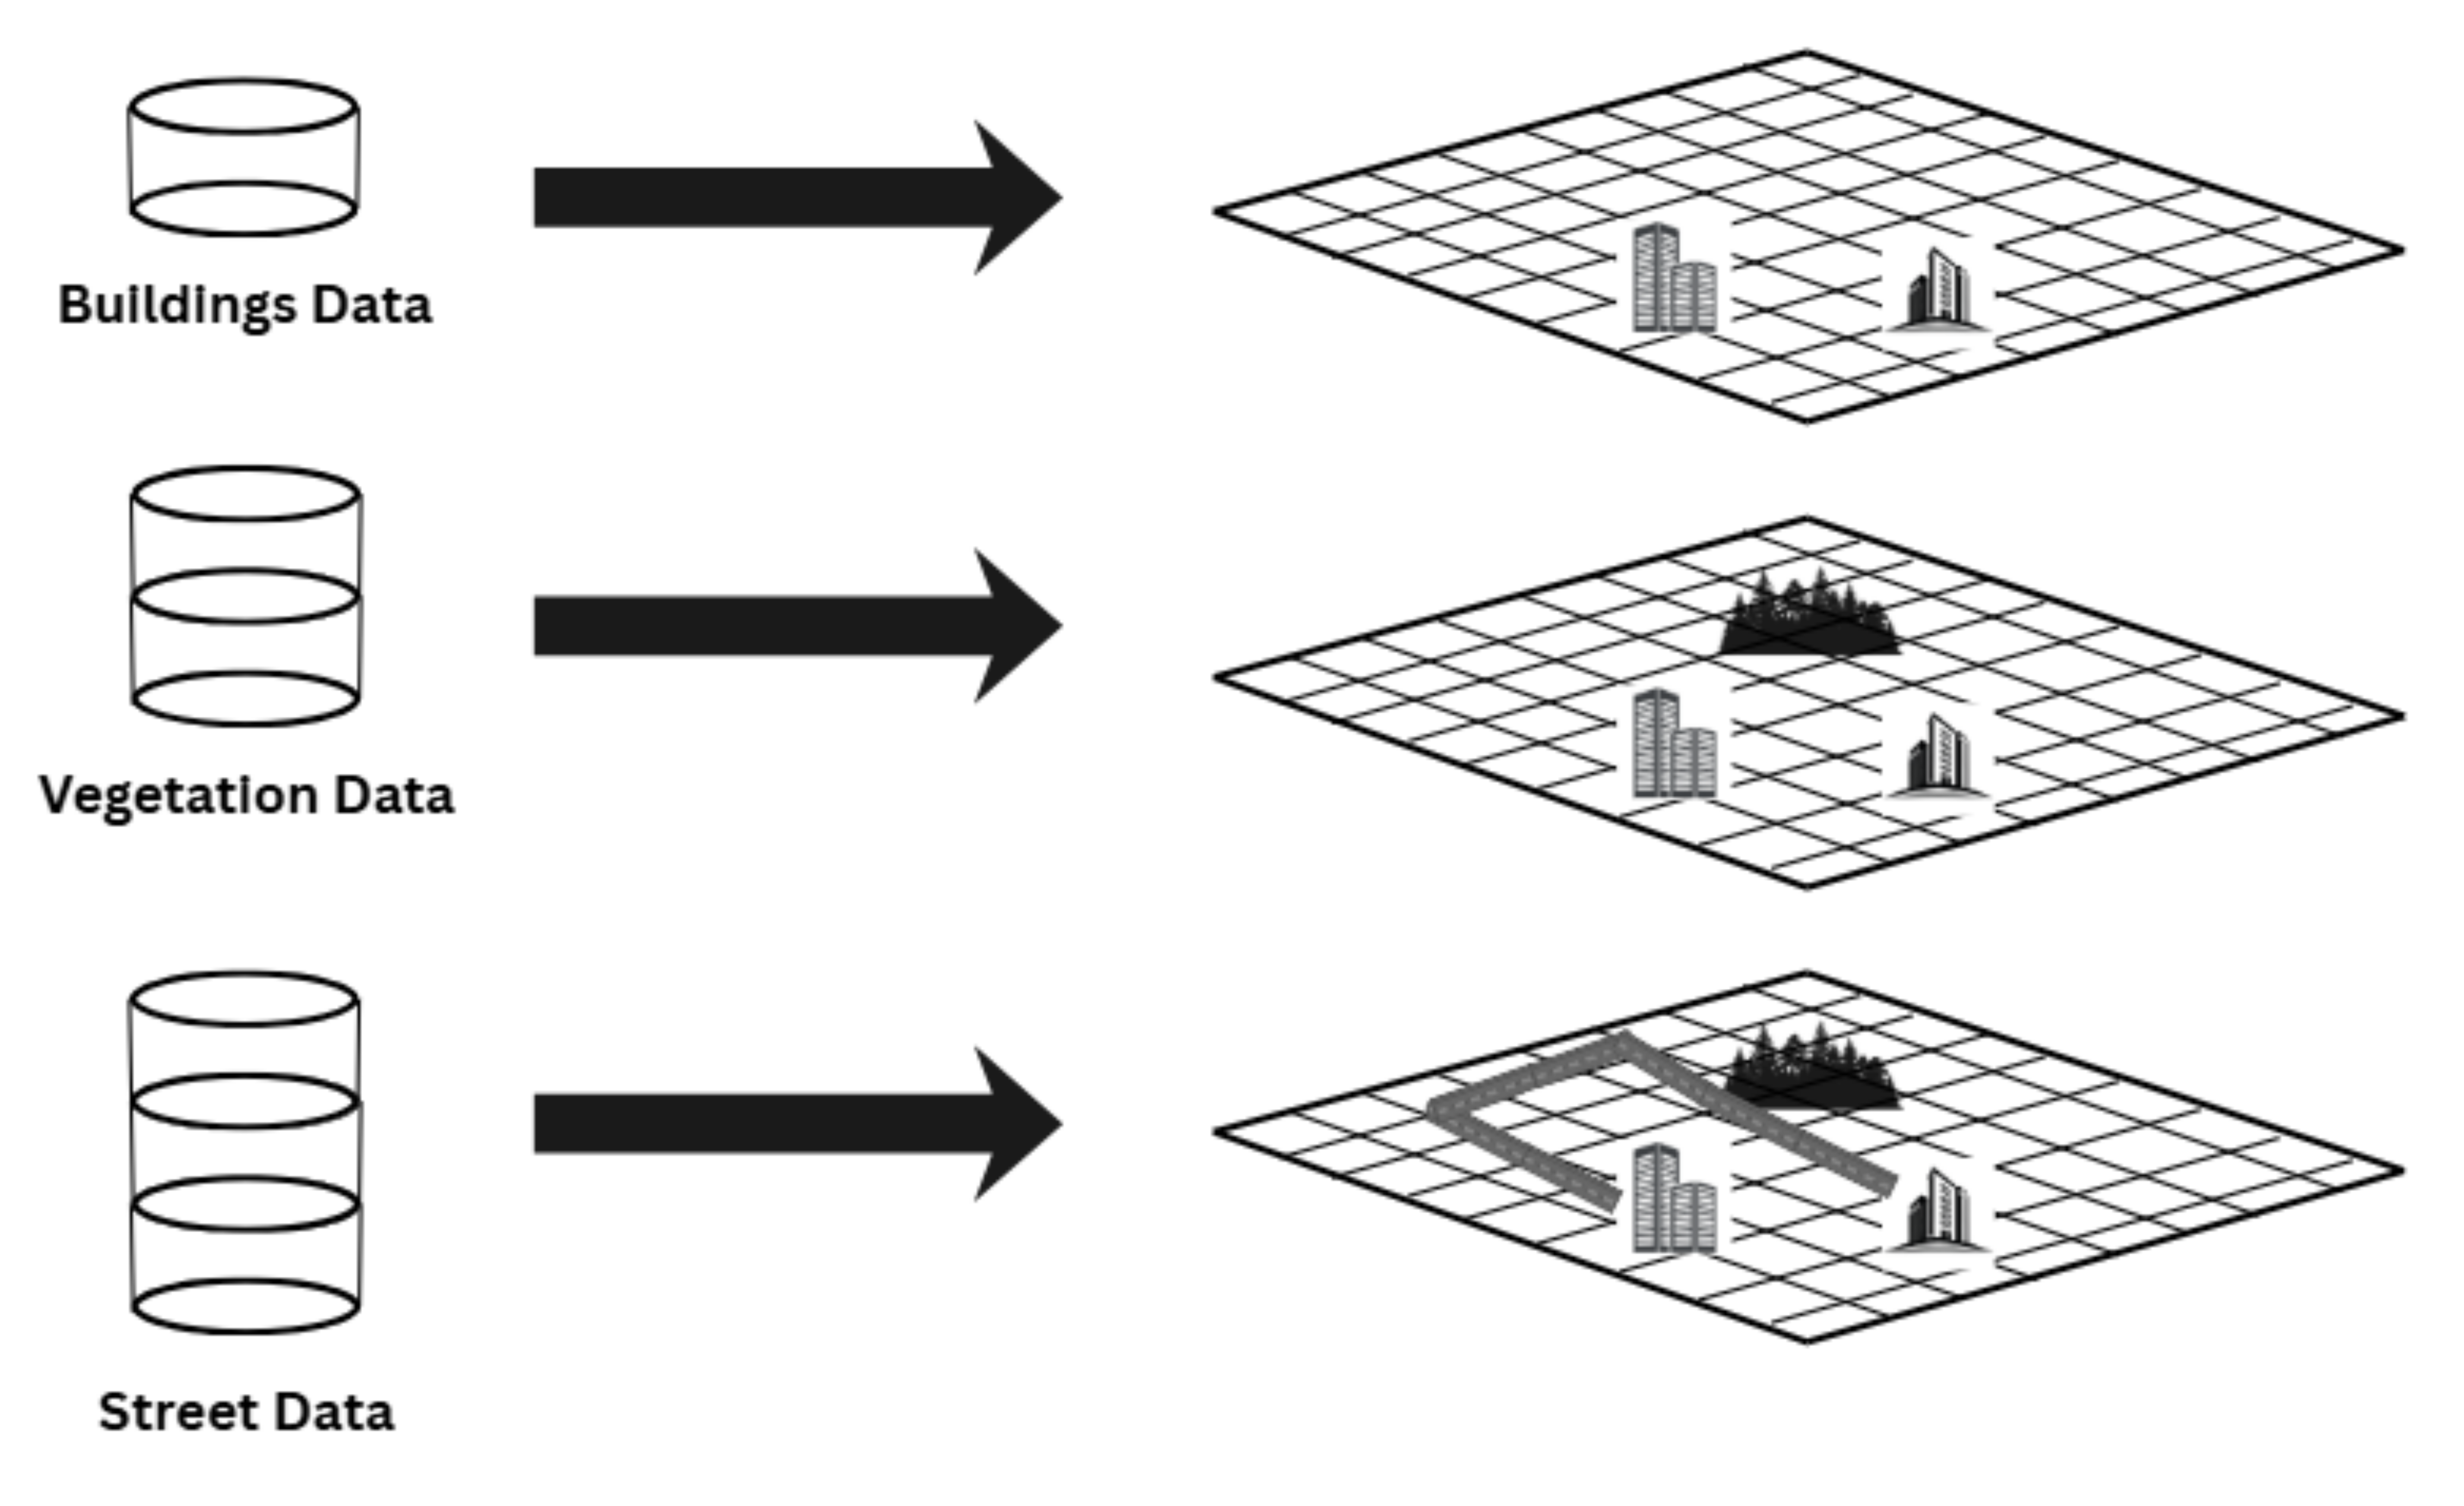
\includegraphics[width=1\textwidth]{image/struktur-GIS.png}
	\caption{Contoh \textit{layer} GIS \autocite{UnitedStatesGeneralAccountingOffice2003}}
	\label{gambar:gis-layers}
\end{figure}

Secara umum, data geospasial pada GIS dipresentasikan dalam dua bentuk utama, yaitu vektor dan raster. Data vektor menyimpan geometri sebagai titik, garis,
atau poligon untuk merepresentasikan objek dalam bentuk diskrit, seperti jalan, gedung, vegetasi, dan lainnya. Sementara itu, data raster memodelkan 
permukaan bumi sebagai \textit{grid} sel dengan suatu resolusi tertentu. Pada Gambar \ref{gambar:gis-layers}, bentuk \textit{layer-layer} digabungkan sehingga memungkinkan operasi analisis
seperti \textit{overlay}, perhitungan jarak, pemotongan wilayah \textit{clip}, dan \textit{resampling} solusi. Pada salah satu contoh studi untuk menganalisis
karhutla, \textcite{Vetrita2025} memanfaatkan GIS untuk menyajikan pemetaan bulanan area terbakar di Indonesia dengan memanfaatkan citra satelit dan serangkaian 
data geospasial sehingga analisis dapat dilakukan untuk melihat deret waktu area terbakar yang konsisten.

\section{Penelitian Terkait}
Untuk memahami lebih dalam terkait permasalahan, studi dilakukan untuk mencari penelitian yang membahas permasalahan dan mencoba memahami langkah solutif
yang telah di uji coba sebagai percobaan penyelesaian masalah. Penelitian yang dilakukan oleh \textcite{Karurung2025} menjelaskan tentang 
kebakaran hutan yang berlokasi di Indonesia dengan fokus pada variasi musiman. Wilayah studi yang dilakukan meliputi provinsi Kalimantan, Sumatra, dan
Papua. Mereka mengembangkan sebuah algoritma ML termasuk RF dan XGBoost dari lima belas faktor kerentanan, seperti 
curah hujan, suhu, kelembapan, indeks vegetasi, topografi, jarak permukiman, hingga keberadaan lahan gambut. Prediksi yang dilakukan berfokus pada
pemetaan tingkat kerentanan kebakaran pada tiga kondisi musim, yaitu hujan, kering, dan gabungan. Hasilnya menunjukkan bahwa model berbasis \textit{ensemble tree}
mampu mencapai akurasi tinggi dengan nilai AUC di atas 0,9 dan mengungkap bahwa pengaruh faktor lingkungan seperti curah hujan dan kelembapan menjadi dominan.

Studi selanjutnya dilakukan dengan melihat penelitian yang dilakukan \textcite{Chen2024} yang memanfaatkan model \textit{Support Vector Machine} (SVM), RF, dan 
\textit{Neural Network} dalam melakukan klasifikasi area \textit{burning} dan \textit{burnt} pada tiga periode waktu (sebelum kebakaran, saat kebakaran, dan setelah kebakaran).
Mereka menggunakan citra Sentinel-1B dan Sentinel-2A untuk mendapatkan citra di lokasi Xintian County, Tiongkok. Fitur yang digunakan merupakan kombinasi dari index vegetasi, 
parameter radar, dan kanal optik. Secara umum, model SVM menunjukkan kinerja paling baik pada fase pra-kebakaran, sedangkan RF dan \textit{Neural Network} memberikan 
hasil yang lebih baik untuk pemetaan area yang sudah terbakar. Studi ini menegaskan bahwa pemilihan algoritma dan fitur citra sangat mempengaruhi kualitas pemetaan
kebakaran berbasis penginderaan jauh (\textit{remote sensing}).

Studi dari \textcite{Abdollahi2023} memberikan pandangan lain tentang prediksi kerentanan kebakaran hutan dengan memberikan pendekatan XAI untuk memberikan penjelasan
dari hasil prediksi. Wilayah studi yang dilakukan berada di Gippsland, Victoria (Australia) dengan menggunakan serangkaian faktor pemicu kebakaran seperti curah hujan, suhu, 
dan topografi. Mereka menggunakan model DL untuk memprediksi kerentanan kebakaran hutan lalu menerapkan metode SHAP untuk menafsirkan kontribusi masing-masing
faktor.  Hasil yang diberikan SHAP mampu menunjukkan fitur-fitur kunci yang mendorong peningkatan kerentanan kebakaran seperti kelembapan, kemiringan lereng, dan jarak ke jalan.
Pendekatan ini memperlihatkan bagaimana XAI dapat mengatasi kasus "\textit{black box}" dalam menjelaskan hasil yang diberikan oleh model prediksi.

Secara keseluruhan, ketiga penelitian tersebut memberikan gambaran penerapan
ML dan XAI pada kasus kebakaran hutan dan lahan. Namun,
eksplorasi pemanfaatan ML dan XAI untuk kebakaran hutan di Asia Tenggara,
khususnya Indonesia, masih relatif terbatas. Integrasi berbagai langkah solutif
seperti pemodelan kerentanan berbasis \textit{ensemble tree}, pemanfaatan berbagai
\textit{raster layer} lingkungan dalam kerangka SIG, serta penerapan XAI yang
terhubung dengan dashboard interaktif belum banyak dikaji secara terpadu. Ruang
inilah yang akan diisi oleh tugas akhir ini.


% \lipsum[1]

% \subsection{Gambar}
% Contoh gambar dapat dilihat pada Gambar \ref{gambar:jaringan}. Gambar dan judulnya diposisikan di tengah. Nomor gambar tidak diakhiri tanda titik. Gambar tersebut dibuat menggunakan aplikasi draw.io dan disimpan ke format PNG setelah dengan zoom setting pada angka 300\%. Ukuran gambar yang ditampilkan dapat diatur dengan mengubah nilai \textit{width} dalam sintaks \textit{includegraphics}.

% \begin{figure}[t] % pilihan opsi yang disarankan: t = top, b = bottom, h = here
% 	\centering
%   \captionsetup{justification=centering}
%     	\includegraphics[width=0.7\textwidth]{image/gambar1.png}
% 	\caption{Contoh gambar jaringan}
% 	\label{gambar:jaringan}
% \end{figure}

% Gambar umumnya tidak jelas atau kabur jika gambar tersebut:
% \begin{enumerate}[a.]
%   \item diperoleh dari hasil cropping pada suatu halaman buku atau situs web;
%   \item hasil pembesaran gambar yang gambar aslinya sebenarnya berukuran kecil; atau
%   \item disimpan dalam resolusi kecil
% \end{enumerate}
% Ketidakjelasan gambar ini dapat dilihat pada garis-garis diagram yang tidak tegas dan tulisan-tulisan dalam gambar yang tampak kabur dan kurang jelas terbaca.

% Untuk mendapatkan gambar yang tidak kabur (\textit{blur}), langkah-langkah berikut dapat digunakan:
% \begin{enumerate}[(a)]
% \item Gambar yang didapat di suatu pustaka atau referensi sebaiknya digambar ulang, misalnya menggunakan PowerPoint, Canva, Figma, draw.io, atau yang lainnya.
% \item Jika diagram atau ilustrasi digambar menggunakan draw.io, saat gambar disimpan ke format PNG atau JPG (\textit{export as}), lakukan \textit{zoom} ke minimal 300\% (\textit{the default value is} 100\%). 
% \item Jika diagram digambar dengan menggunakan PowerPoint, gambar dapat langsung di-\textit{copy-paste} ke Word.
% \end{enumerate}

% \subsection{Tabel}
% Tabel ada dua jenis, yaitu tabel yang bisa termuat dalam satu halaman dan tabel yang sangat panjang sehingga tidak muat dalam satu halaman.
% \subsubsection{Tabel yang Muat dalam Satu Halaman}
% Contoh tabel dapat dilihat pada Tabel \ref{tbl:harga1} dan \ref{tbl:harga2}. Tabel dan judulnya dibuat rata kiri dan judul tabel diletakkan di atas tabel. Usahakan tabel dapat ditulis dalam satu halaman, tidak terpotong ke halaman berikutnya.

% \begin{table}[t] % pilihan opsi yang disarankan: t = top, b = bottom, h = here
%   \begin{tabular}{ | p{2cm} | p{2cm} | p{3cm} |}
% 	\hline
% 	Nama 	& Satuan 		& Harga \\
% 	\hline
% 	Buku 	& Exemplar	& 25000 \\
% 	Komputer	& Unit		& 2500000 \\
% 	Pensil	& Buah		& 118900 \\
% 	\hline
% 	\end{tabular}
% \caption{Tabel harga bahan pokok}
% \label{tbl:harga1}
% \end{table}



% \begin{table}[t] % pilihan opsi yang disarankan: t = top, b = bottom, h = here
% 	\begin{tabular}{ | l | c | r | }
% 	\hline
% 	Nama 	& Satuan 		& Harga \\
% 	\hline
% 	Buku 	& Exemplar	& 25000 \\
% 	Komputer	& Unit		& 2500000 \\
% 	Pensil	& Buah		& 118900 \\
% 	\hline
% 	\end{tabular}
% \caption{Tabel harga bahan sekunder}
% \label{tbl:harga2}
% \end{table}

% % -- Example of importing table from external file --
% \subsubsection{Mengimpor Tabel dari Berkas Eksternal}

% Tabel \ref{tbl:harga3} diimpor dari berkas eksternal \textit{table/tabel1.tex} menggunakan perintah \textit{input}. 
% Dengan demikian, jika tabel tersebut perlu diubah, cukup mengubah pada berkas eksternal tersebut tanpa perlu mengubah pada berkas utama ini.

% \input table/tabel1.tex


% % -- Example of long table --
% \subsubsection{Tabel yang Sangat Panjang}
% Jika tabel terlalu panjang sehingga tidak muat dalam satu halaman, gunakan paket 
% \textit{longtable} untuk membuat tabel yang dapat terpotong ke halaman berikutnya, 
% seperti pada Tabel \ref{tbl:longtable1}.

% \begin{longtable}{@{\extracolsep{\fill}} l c r r}
% \caption{Comprehensive Data Table Example}\label{tbl:longtable1} \\
% \toprule
% \textbf{ID} & \textbf{Name} & \textbf{Score} & \textbf{Rank} \\
% \midrule
% \endfirsthead

% \caption{Comprehensive Data Table Example (lanjutan)} \\
% \toprule
% \textbf{ID} & \textbf{Name} & \textbf{Score} & \textbf{Rank} \\
% \midrule
% \endhead

% \midrule
% \multicolumn{4}{r}{\textit{Bersambung ke halaman berikutnya}} \\
% %\bottomrule
% \endfoot

% \bottomrule
% \endlastfoot

% % === Table Data ===
% 1 & Alice Smith & 89 & 5 \\
% 2 & Bob Johnson & 93 & 3 \\
% 3 & Carol Davis & 95 & 2 \\
% 4 & Daniel Wilson & 88 & 6 \\
% 5 & Eve Thompson & 97 & 1 \\
% 6 & Frank Brown & 85 & 7 \\
% 7 & Grace Lee & 91 & 4 \\
% 8 & Henry Miller & 80 & 9 \\
% 9 & Irene Garcia & 83 & 8 \\
% 10 & Jack Robinson & 78 & 10 \\
% % Repeat with more rows to make it long
% 11 & Kevin Harris & 76 & 11 \\
% 12 & Laura Martin & 75 & 12 \\
% 13 & Michael Clark & 74 & 13 \\
% 14 & Natalie Lewis & 73 & 14 \\
% 15 & Olivia Walker & 72 & 15 \\
% 16 & Peter Hall & 71 & 16 \\
% 17 & Quinn Allen & 70 & 17 \\
% 18 & Rachel Young & 69 & 18 \\
% 19 & Samuel King & 68 & 19 \\
% 20 & Tina Wright & 67 & 20 \\
% 21 & Uma Scott & 66 & 21 \\
% 22 & Victor Green & 65 & 22 \\
% 23 & Wendy Adams & 64 & 23 \\
% 24 & Xavier Nelson & 63 & 24 \\
% 25 & Yolanda Carter & 62 & 25 \\
% 26 & Zachary Perez & 61 & 26 \\
% 27 & Amelia Baker & 60 & 27 \\
% 28 & Benjamin Rivera & 59 & 28 \\
% 29 & Charlotte Rogers & 58 & 29 \\
% 30 & David Murphy & 57 & 30 \\
% 31 & Ethan Cooper & 56 & 31 \\
% 32 & Fiona Reed & 55 & 32 \\
% 33 & George Bailey & 54 & 33 \\
% 34 & Hannah Cox & 53 & 34 \\
% 35 & Isaac Howard & 52 & 35 \\
% 36 & Julia Ward & 51 & 36 \\
% 37 & Kyle Flores & 50 & 37 \\
% 38 & Lily Bell & 49 & 38 \\
% 39 & Mason Sanders & 48 & 39 \\
% 40 & Nora Patterson & 47 & 40 \\
% 41 & Owen Ramirez & 46 & 41 \\
% 42 & Penelope Torres & 45 & 42 \\
% 43 & Quentin Foster & 44 & 43 \\
% 44 & Rebecca Gonzales & 43 & 44 \\
% 45 & Sebastian Bryant & 42 & 45 \\
% 46 & Taylor Alexander & 41 & 46 \\
% 47 & Ursula Russell & 40 & 47 \\
% 48 & Vincent Griffin & 39 & 48 \\
% 49 & William Diaz & 38 & 49 \\
% 50 & Zoe Simmons & 37 & 50 \\
% % (You can easily extend this list to hundreds of rows)
% \end{longtable}

% \subsubsection{Beberapa Contoh Penulisan Rumus atau Persamaan Matematika Menggunakan LaTeX Termasuk Penomorannya}
% Contoh rumus matematika dapat ditulis seperti pada Persamaan \ref{eq:contoh1} di bawah ini. 
% Penomoran persamaan diletakkan di sebelah kanan, dan rumus ditulis dalam mode \textit{display math}.
% \begin{equation}
% E = mc^2
% \label{eq:contoh1}
% \end{equation}

% Contoh lain penulisan rumus matematika yang lebih kompleks dapat ditulis seperti pada Persamaan \ref{eq:rumus2}.

% \begin{align}
% f(x) &= ax^2 + bx + c \\
% f'(x) &= \frac{d}{dx}(ax^2 + bx + c) \notag \\ % tidak menampilkan nomor pada baris ini
%       &= 2ax + b \label{eq:rumus2}
% \end{align}

% Jika rumus terlalu panjang untuk ditulis dalam satu baris, gunakan lingkungan \textit{multline} seperti pada Persamaan \ref{eq:rumus3} di bawah ini.
% \begin{multline} 
% y = a_0 + a_1x + a_2x^2 + a_3x^3 + a_4x^4 + a_5x^5 + a_6x^6 + a_7x^7 \\
%     + a_8x^8 + a_9x^9 + a_{10}x^{10} \label{eq:rumus3}
% \end{multline}

% Jika ada penurunan rumus yang terdiri dari beberapa baris, namun tidak memerlukan penomoran pada setiap baris, gunakan lingkungan \textit{align*}, misalnya:

% \begin{align*} 
% S &= \sum_{i=1}^{n} i^2 \\
%   &= 1^2 + 2^2 + 3^2 + \cdots + n^2 \\
%   &= \frac{n(n + 1)(2n + 1)}{6}
% \intertext{Contoh lainnya adalah rumus untuk mencari nilai rata-rata fungsi $f(x)$ pada interval $[p, q]$:}
% \bar{f} &= \frac{1}{q - p} \int_{p}^{q} f(x) \, dx \\
%         &= \frac{1}{q - p} \int_{p}^{q} (ax^2 + bx + c) \, dx \\
%         &= \frac{1}{q - p} \left[ \frac{a}{3}x^3 + \frac{b}{2}x^2 + cx \right]_p^q \\
%         &= \frac{a(q^3 - p^3)}{3(q - p)} + \frac{b(q^2 - p^2)}{2(q - p)} + c \label{eq:rumus4}
% \end{align*}



% \subsection{Algoritma, Pseudocode, atau Kode}
% Contoh penulisan algoritma atau pseudocode dapat ditulis seperti pada Kode \ref{alg:contoh1} di bawah ini. 
% Gunakan paket \textit{listings} untuk menulis source code dalam bahasa pemrograman tertentu, seperti pada Kode \ref{lst:contoh1}. 


% % -- Example of pseudocode and source code listing --
% % -- Gunakan minipage agar listing tidak terpotong ke halaman berikutnya --
% \begin{minipage}{\textwidth} 
% \begin{lstlisting}[frame=lines, captionpos=t, caption={Contoh pseudocode}, label={alg:contoh1}]
% ALGORITHM HelloWorld
%    PRINT "Hello, World!"
% END ALGORITHM
% \end{lstlisting}
% \end{minipage}

% \begin{minipage}{\textwidth}
% \begin{lstlisting}[language=Python, frame=single, caption={Contoh source code Python}, captionpos=t, label={lst:contoh1}]
% def hello_world():
%     print("Hello, World!")       
% hello_world()
% \end{lstlisting}
% \end{minipage}


% \section{Beberapa Kesalahan Penulisan yang Sering Terjadi}
% \subsection{Penggunaan Kata "di mana" atau "dimana"}
% Banyak yang menuliskan kata "di mana" atau "dimana" sebagai pengganti kata "which" dalam bahasa Inggris. 
% Padahal, penggunaan kata "di mana" atau "dimana" tidak tepat dalam konteks tersebut. Demikian juga untuk kata serupa, misalnya "yang mana".
% Kata "di mana" atau "dimana" ini harus diganti dengan kata lain, seperti "dengan", "tempat", "yang", dan sebagainya tergantung kalimatnya.
% Penjelasan lengkap dapat dilihat pada \autocite{BPBI}.

% \subsection{Penggunaan Kata "sedangkan" dan "sehingga"}

% \begin{table}[t]
%   \begin{tabular}{|c|l|l|}
%   \hline
%   Kata & Salah & Benar \\ \hline
%   sedangkan & \begin{tabular}[c]{@{}c@{}}Sedangkan sistem lama masih\\ digunakan oleh banyak pengguna.\end{tabular} & \begin{tabular}[c]{@{}c@{}}Sistem lama masih digunakan\\ oleh banyak pengguna,\\ sedangkan sistem baru belum siap.\end{tabular} \\ \hline
%   sehingga & \begin{tabular}[c]{@{}c@{}}Sehingga sistem lama masih\\ digunakan oleh banyak pengguna.\end{tabular} & \begin{tabular}[c]{@{}c@{}}Sistem lama masih digunakan\\ oleh banyak pengguna sehingga\\ sistem baru belum siap.\end{tabular} \\ \hline
%   \end{tabular}
%   \caption{Contoh penggunaan kata "sedangkan" dan "sehingga"}
%   \label{tbl:sedangkan_sehingga}
% \end{table}

% Kata "sedangkan" dan "sehingga" adalah kata hubung atau konjungsi. 
% Konjungsi adalah kata atau ungkapan yang menghubungkan satuan bahasa 
% (kata, frasa, klausa, dan kalimat). 
% Konjungsi dapat dibagi menjadi konjungsi intrakalimat dan antarkalimat.  
% Kata "sedangkan" menghubungkan dua klausa yang bersifat kontrasif, 
% sedangkan "sehingga" menghubungkan dua klausa yang bersifat kausal. 
% Dalam ragam formal, kata hubung “sedangkan” dan “sehingga” hanya dapat digunakan 
% sebagai konjungsi intrakalimat sehingga kedua konjungsi itu \textbf{tidak dapat diletakkan pada awal kalimat}.
% Selain itu, penggunaan kata "sedangkan" harus didahului oleh koma (,), sedangkan kata "sehingga" tidak perlu didahului oleh koma (,).
% Contoh penggunaan yang benar dan salah dapat dilihat pada Tabel \ref{tbl:sedangkan_sehingga}.


% \subsection{Penggunaan Istilah yang Tidak Baku}
% Ada beberapa istilah yang sering digunakan dalam pembicaraan sehari-hari, tetapi tidak baku dalam penulisan ilmiah.
% Beberapa istilah tersebut antara lain:
% \begin{enumerate}
%   \item analisa $\rightarrow$ analisis
%   \item eksisting atau existing $\rightarrow$ yang ada atau saat ini
%   \item bisnis proses $\rightarrow$ proses bisnis
%   \item user $\rightarrow$ pengguna
%   \item system $\rightarrow$ sistem
%   \item database $\rightarrow$ basis data
%   \item aktifitas $\rightarrow$ aktivitas
%   \item efektifitas $\rightarrow$ efektivitas
%   \item sosial media $\rightarrow$ media sosial
% \end{enumerate}

% \subsection{Pemisah Desimal dan Ribuan}
% Tanda pemisah desimal dalam bahasa Indonesia adalah tanda koma, contoh:
% \begin{enumerate}
%   \item (Salah) Akurasi naik menjadi 50.6\% 
%   \item (Benar) Akurasi naik menjadi 50,6\% 
% \end{enumerate}

% \subsection{Daftar atau \textit{List}}
% Ada beberapa aturan penulisan daftar atau \textit{list} yang perlu diperhatikan, antara lain:
% \begin{enumerate}[(a)]
% \item Jika memungkinkan, hindari penggunaan “bullet points” atau sejenisnya. Sebaiknya, gunakan angka (1, 2, 3, ...) atau huruf (a, b, c, …). Dengan demikian, pembaca dapat dengan mudah melihat jumlah \textit{item} atau \textit{list}. 
% \item Jika dalam daftar hanya ada satu item, tidak perlu menggunakan nomor urut.
% \item Penjelasan atau deskripsi suatu item sebaiknya menyatu dengan judul item tersebut, tidak berbeda halaman. Contoh yang salah: judul item ada di halaman 10, namun deskripsinya di halaman 11. Sebaiknya pindahkan judul tersebut ke halaman 11.
% \item Jika penjelasan atau deskripsi suatu item cukup panjang, misalnya lebih dari 1 halaman atau terdiri atas beberapa paragraf, sebaiknya setiap item tersebut dijadikan judul subbab, kecuali jika level subbab sudah mencapai level 4. 
% \end{enumerate}

% \subsection{Penggunaan Kata "masing-masing" dan "setiap"}
% Kata “masing-masing” digunakan di belakang kata yang diterangkan, misalnya 
% "Setiap proses menggunakan algoritma masing-masing". Kata “tiap-tiap” atau “setiap”
% ditempatkan di depan kata yang diterangkan, misalnya
% "Setiap proses menggunakan algoritma tertentu".
